\chapter{Prototype Implementation}
\label{chap:prototype}

To give a proof of concept, we implemented a prototype which shows a good selection of the functionality expected by the Healthbank system. The prototype is intended to show the possibilities of such a system as well as to build a solid basis on which future work can build upon. In the remainder of this chapter we discuss in detail the data model, architecture and technologies used for implementing the prototype.


%%% ------------- SECTION -------------

Because of the extensibility and reusability constraint on the system, we decoupled the implementation of the server and client into two completely separated projects. The server has direct access to the MongoDB~\cite{MongoDB} database via a socket connection on the localhost. The connection between client and server is done via HTTP and AJAX requests to the server REST API. In figure \ref{fig:prototypeSetup} we illustrate this relation.

% Figure 4.1
\begin{figure}[h]
%\centering
%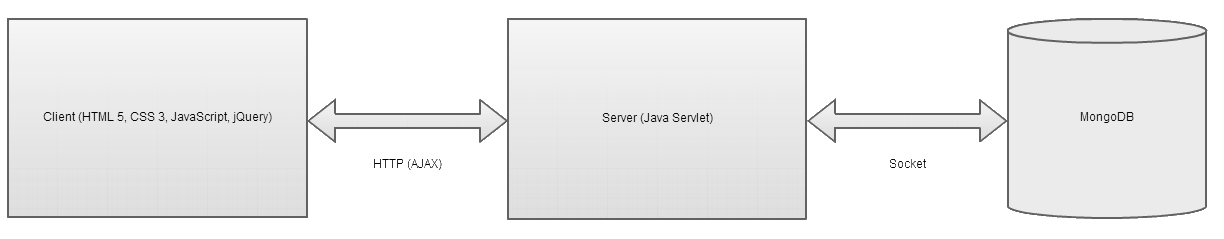
\includegraphics[width=408px,height=80px]{prototypeSetup.png}
\makebox[\textwidth][c]{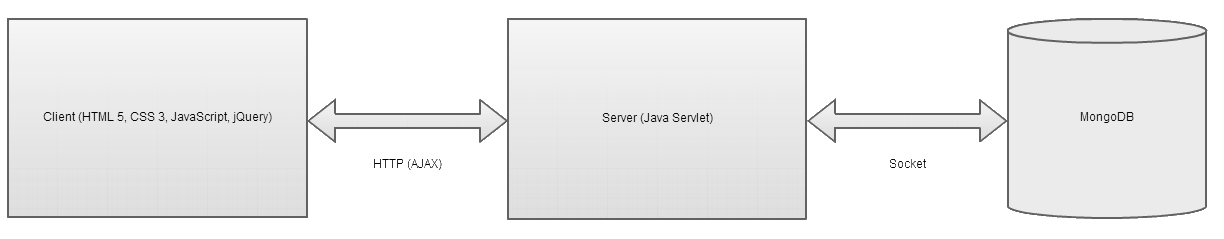
\includegraphics[width=408px,height=80px]{prototypeSetup.png}}%
\caption{Components of the prototype.}
\label{fig:prototypeSetup}
\end{figure} 


%%% ------------- SECTION -------------
\section{Data Model}

As supposed, we used an instance of MongoDB~\cite{MongoDB}, which is open-source, agile, scalable and one of the leading NoSQL databases at the moment. The JSON-style~\cite{JSON}, document-oriented storage works very well for our purposes, since we can use JSON as the main communication format for our AJAX calls between server and client. \newline
The following table \ref{tab:collectionTable} describes all the collections (equivalent of an RDBMS table) used in the MongoDB instance to support our functionalities:\newline

\begin{table}[h]
  \centering
	\begin{tabular}{l l}
	Collection name & Description \\
	\hline
	applications & Contains application specific information. \\
	 & Icons are saved in applications.files collection.\\
	circles & Contains all information about user`s circles \\
	messages & Contains messages sent between users \\
	news & Contains news entries \\
	records & Contains all health record related data. \\
	 & Files are saved in records.files collection. \\
	spaces & Contains all information about user`s spaces \\
	users & Contains all user related data such as name, address etc. \\
	 & Icons are saved in users.files collection.\\
	\end{tabular}
	\caption{The list of collections used on the MongoDB instance}
  \label{tab:collectionTable}
\end{table}

Every entry in a collection contains an ObjectID which identifies the object uniquely within the database. The more every entry has a field called \emph{timedate} which holds the time and date of the object creation. As it is a MongoDB database, all data is saved as JSON and hence in a key-value style. Here is an example of a message collection entry representing a message sent from one user to another.\newline

\begin{lstlisting}[language=json,firstnumber=1]
{
        "_id" : ObjectId("id"),
        "message" : "This is the first ever test message. Fingers crossed...",
        "read" : "true",
        "recipientID" : "id",
        "senderID" : "id",
        "subject" : "The first message of all time",
        "timedate" : "07/11/2013 12:50:47"
}
\end{lstlisting}

The \emph{ID} fields contain the mentioned ObjectID values of the respective user. Such an ObjectID values is composed of the current time, machine id, a process id and a random value.

%%% ------------- SECTION -------------
\section{Concepts}

In this section we describe the concepts used in the prototype to implement the requirements from chapter \ref{chap:generaldesign}. 

\subsection{Login and Session Management}\label{loginSession}

Authentication and session management is generally a very tricky task. For the prototype we decided to apply a rather simplistic but solid method. This method omits cookies and builds on top of the new HTML5 storage possibilities, especially the local storage~\cite{localstorage}.

The user needs at least a unique user name and a password to register. When the login with user name and password was successful, the system will generate a session key for the user and set an expiration time for the key. The session is set to expire after one hour of inactivity. With every request to the API by the user, the session key has to be provided as well as a credentials value. These credentials are the composition of the user name and password in a hashed form for security purposes. The session key and the credentials value are stored locally on the client device and are read by every call to the REST API. If the session has expired or there was any other issue, the user is automatically passed on to the login page. 

\subsection{Circle}

The concept of circles is one of the most essential in our system. Circles are what we called access categories in chapter \ref{chap:generaldesign} and allow the user to share any record with other users such as friends and family or doctors and hospitals. The concept is in many ways similar to the one used by Google for their social media platform Google+~\cite{googlePlus}. We chose to adapt Googles concept, because we like it and we think that this way it will be easier for the user to get used to it, compared to something new and unique. \newline
There are two aspects to circles which needed to be considered in the prototype. Firstly, there is the creation and manipulation of circles as well as the assignment of other users to them. Secondly, is the assignment of record entries to circles. In the GUI these two aspects are separated but logically they are highly coupled. All the record entries assigned to a certain circle are automatically visible by users assigned to the very same circle. 

On the webpage we designed a dedicated page for the circle management (see figure \ref{fig:circlesScreenshot}). On this page the user will see four predefined circles for $Family$, $Friends$ as well as $Medical Professionals$ and $Wellness Professionals$. These four circles are fixed and the user cannot delete or change them apart from their colour. By clicking on the circle with a $+$ sign in the centre the user can add a new circle. A circle consists of a name, a description and a colour for illustration purposes. User created circles can be edited and deleted. To see the users in a circle or to edit one, the user can click on them. As a result of a click we will show a list of rectangles containing the user icons and names of the users present in the circle as illustrated in figure \ref{fig:circlesScreenshot}.  The more, next to this list there are buttons to edit and delete (only on user generated circles) the circle as well as to add spaces (see next subsection \ref{spaces}) to a circle. This last button actually allows the user to add all records who were assigned to this circle, and will be assigned to it in future, to the specified space. Spaces are the implementation of the concept of folders and will be explained in the next subsection. The rectangles in the list have drag-and-drop support which can be used to move them to the trash (remove a user) as well as to assign them to other circles (by dropping on a circle). To find users in the first place the circles page also contains a search field on top which allows to find users by user, first, last or company name as well as by email. 

% Figure 4.2
\begin{figure}[h]
%\centering
%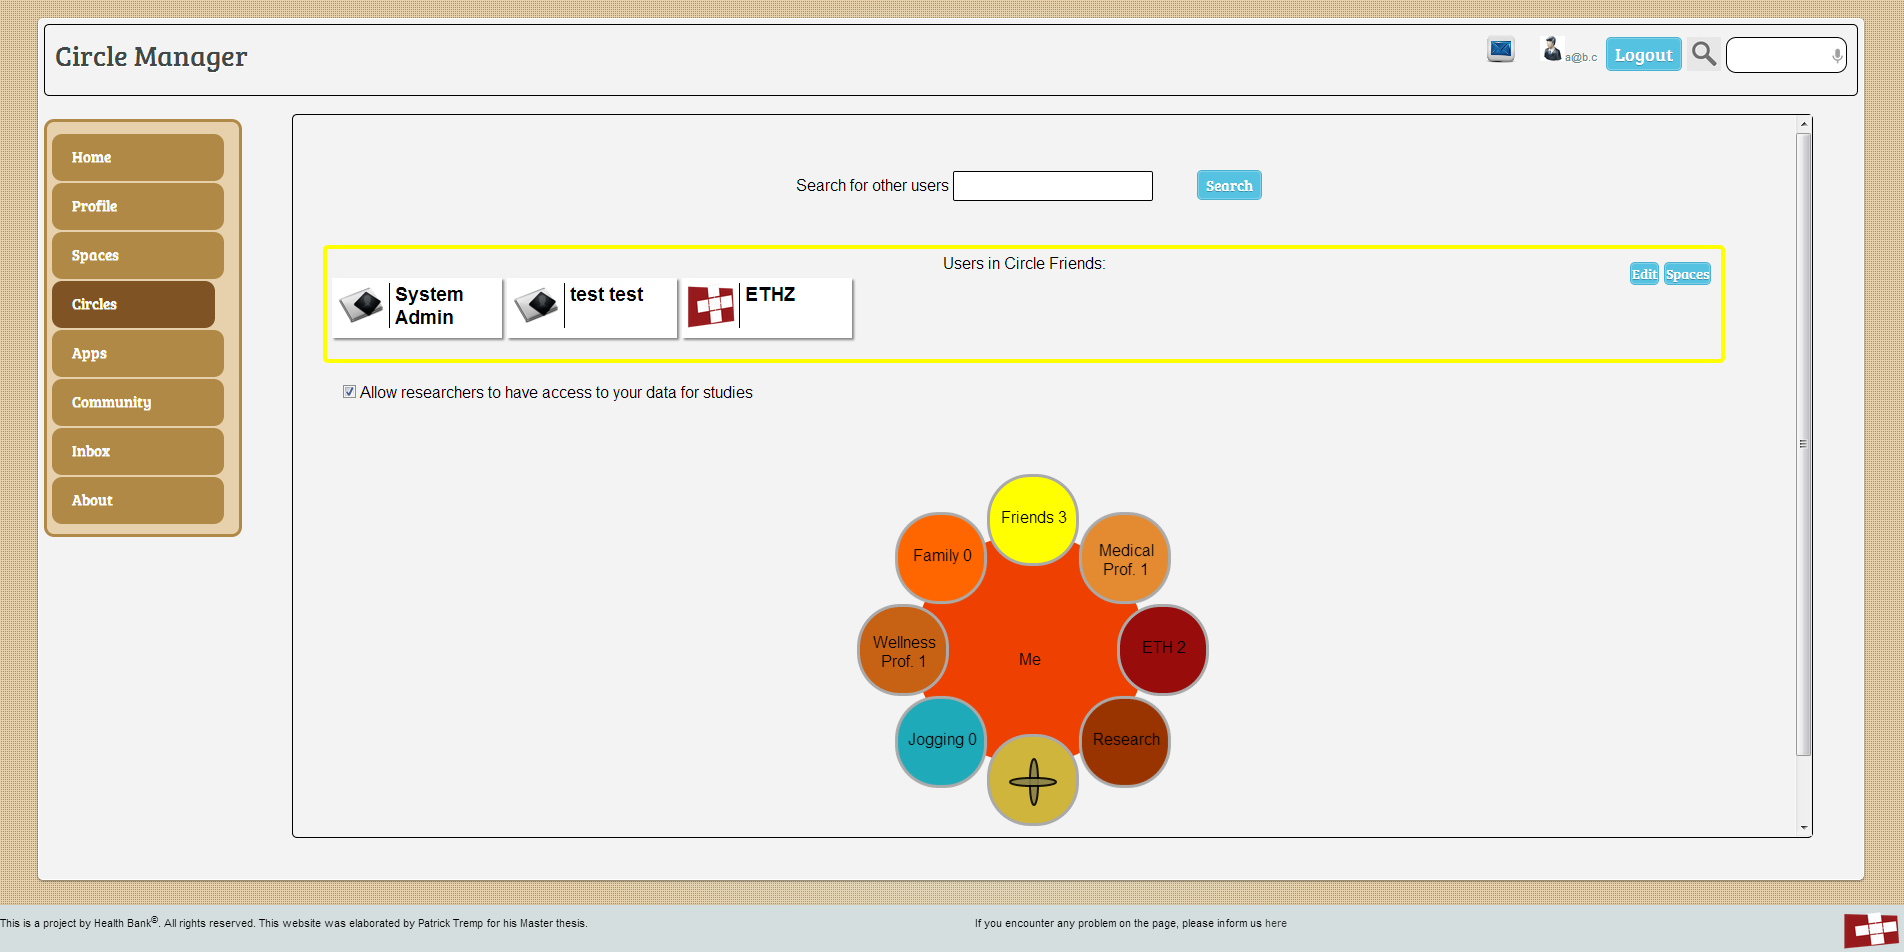
\includegraphics[width=476px,height=238px]{circlesScreen.png}
\makebox[\textwidth][c]{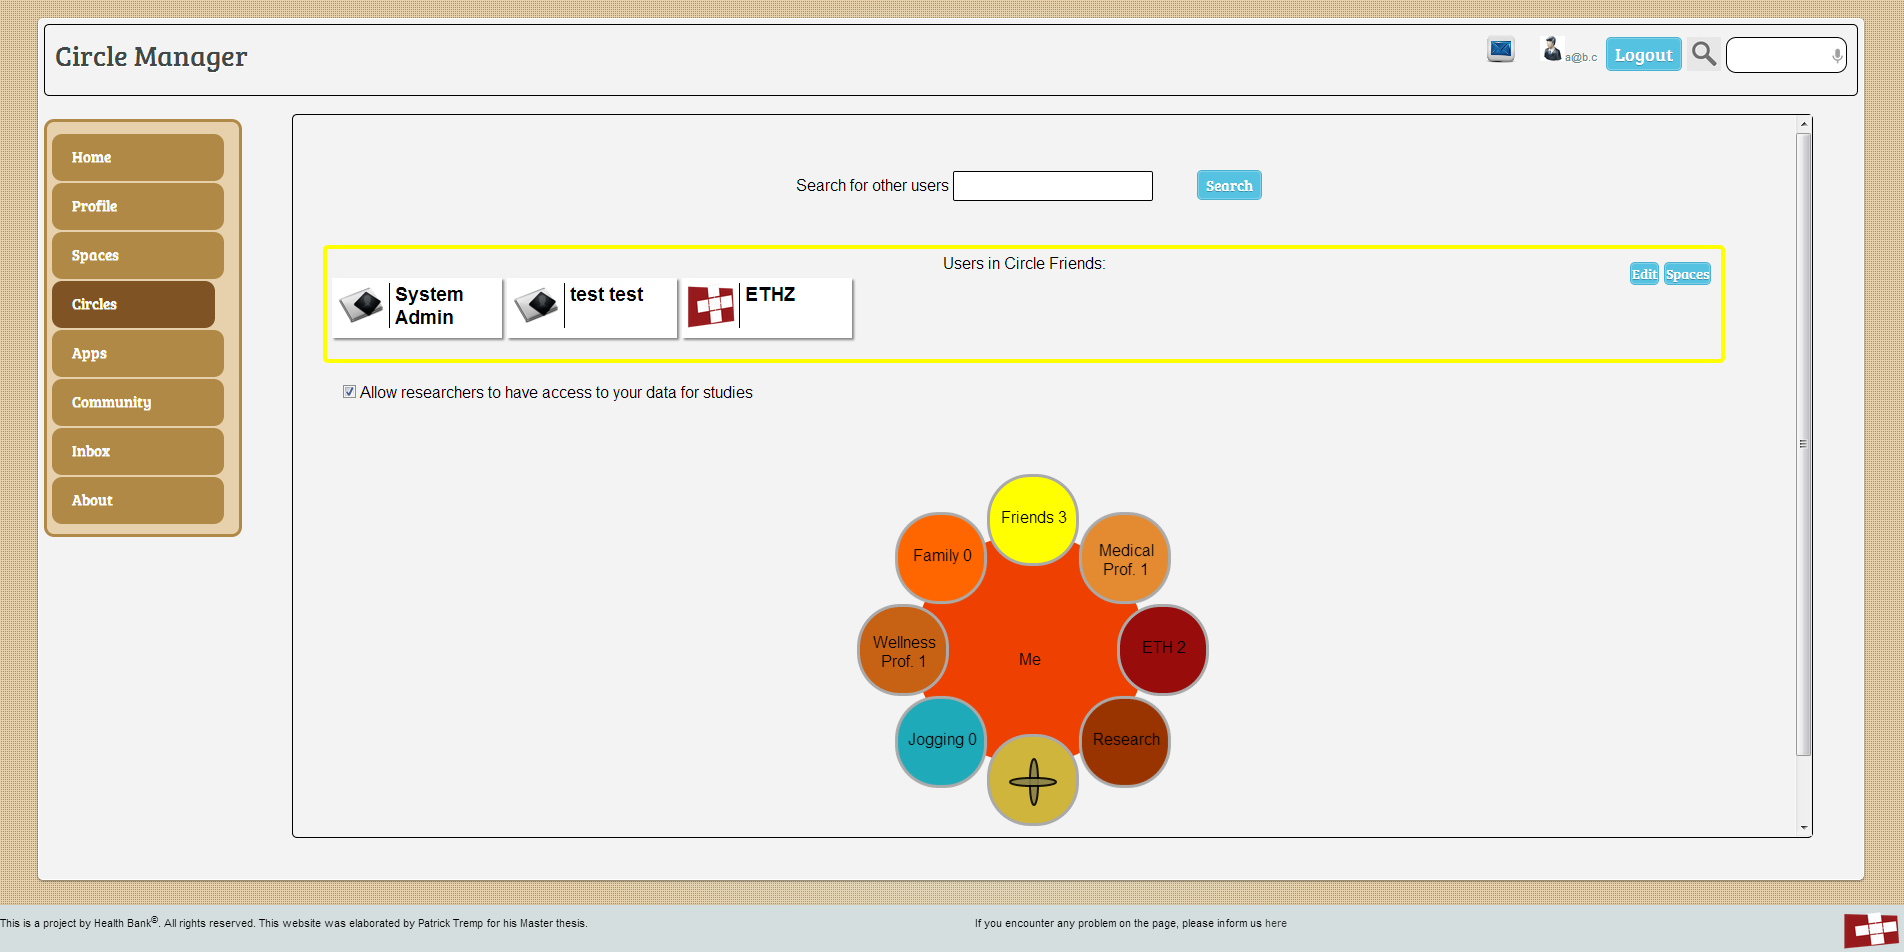
\includegraphics[width=476px,height=238px]{circlesScreen.png}}%
\caption{Screenshot of the circles page in the prototype}
\label{fig:circlesScreenshot}
\end{figure} 


\subsection{Spaces}\label{spaces}

In chapter \ref{chap:generaldesign} we defined the concept of folders. For the prototype we called this concept spaces. Generally speaking a space is a set of entries in a user`s health record. Additionally a user $A$ can also put entries from other users, who shared some entries with $A$, into its spaces. Nevertheless spaces are always bound to one user and other users are not allowed to see or change $A$`s spaces. Besides the list of record entries assigned to the space, a space can also contain a visualization. This visualization will get all the record entries in the space as input and may use them to create beautiful illustrations. 

Users control their spaces in the spaces page of the prototype. Whenever the user clicks on the spaces link in the navigation, the so called $All Space$ will be shown, which contains all the recent record entries of the user. This \emph{all} space is similar to the Twitter feed of a user or the Facebook chronicle. \newline
On top of the list there is a dropdown menu for filtering. Filtering allows the users to inspect record entries of users who shared their data with them. In this menu the user can select other user individually or even entire circles. By selecting $no filter$ all users from $A$`s circles will be selected. The selection of another user $B$ in the filter dropdown has the consequence that all the entries, which $B$ has shared with $A$, will appear on the list. By selecting an entire circle, all the entries, which the users in that circle shared with $A$, will appear on the list. Entries by other users will be indicated as such by a colouring system. It is possible that a user will not see any record entries of $B$ when $B$ is selected in the filtering menu. This can happen, when $B$ does not share anything with $A$. The filtering menu will be present in all of the different spaces. In all but the \emph{all} space there is the additional restriction, that only entries of other users will be shown, which $A$ has assigned to the particular space.

At the very top of the spaces page there are multiple tabs for navigation between the different spaces. The user can control the order in which the spaces appear in this tab list, create new spaces and edit them by clicking on the gear icon at the right hand side. A space is defined by a name and a description and can optionally contain a visualization. An additional feature allows to hide spaces, which the user currently does not use, on the tab list. This helps the users to keep the list clean and short. 


\subsection{Profile}
As described before the profile of a user has to contain at least a user name and a password. The more, we ask for the first and last name in the registration process. Once logged into the system, the user can visit the profile page any time and edit its data. Besides properties like the address, phone numbers, insurance type etc., users can also change their user icon and password. For institute users the profile page looks slightly different. Rather than detailed information about the individual user, institutes can enter a description of the company including what the company is known for, opening hours etc. Also on the profile page the users can decide to which circles they like to share its profile data. So far we have an all or nothing policy. Either the user shares all its profile data with its selected circle or only what is publicly visible. Publicly available are the user`s name as well as the user icon. This data is shown e.g. when a user searches for other users. The detail view opens when you click on a user entry. Depending on whether or not you are in one of the circles, this other user selected for profile sharing, this detail page will show only the public or all profile data. 

Technically we solved the profile sharing by storing user data twice. Usually all profile data is stored in the users collection of the database as described in the collection list above. Non critical fields, such as the users first and last name, the icon, the address, phone numbers, email etc., are then additionally stored as an entry in the users health record. This entry gets updated each time the profile is updated. By doing so we can now apply circle information to that entry and share this with other users. In other words the profile information stored in the users collection is not accessed for showing user`s details. Hence, no sensitive data such as the password, session key or similar is ever visible for other users.


\subsection{Applications}

In the prototype the user can access the application section via the navigation. Patients will be able to go to the market, where all the applications and visualizations are listed and their details can be inspected. The more, they can access a list of all the applications as well as visualizations which they have already installed to their account. Institute users on the other hand have some more possibilities. They can add new applications or visualizations, see and edit the applications and visualizations they have already contributed to the system and inspect the developer guide. 

In the prototype applications contain a name, a description and an icon. Furthermore, the author can specify a version number, define if the application is on- or offline (visible in the market or only accessible by the author) and for whom the application was built for (users, institutes or both). The applications have to be written in HTML with the help of CSS and JavaScript. To keep matters separated, the author can upload individual files for HTML, CSS and JavaScript content. Once the application is in the system the author can edit the information and populate a field called 'what is new'. With this field the author can tell the clients what has changed in comparison to the last version, similar to the Android market. When a new application is uploaded, it gets a unique identification as well as an application secret. These values are only visible for the author. The secret is needed for B2B communication and can be refreshed if needed. 

Once the user has seen the details of an application and hit the install button, the application can be accessed by clicking on them. The application code is loaded into an iframe component on the page and runs from there. As mentioned in chapter \ref{chap:generaldesign}, we provide two methods for adding new entries to the user`s record. The straight forward way is the manual insertion of the entry by the user. With this method the user enters data directly from within the application running in the iframe while the user is already logged in and has a valid session key. This information is used by the client API to access the server and add the entry to the record. The second method allows business to business communication from the third-party server directly to our server. During this process no user needs to be logged in. Therefore we needed to come up with a different authentication solution for B2B communication. The solution, we have chosen, is illustrated in figure \ref{fig:b2b}. Illustrated as $1)$ in the figure is the process of installing the application on our system. When the user installs the application and opens it on the Healthbank GUI, we expect that the application shows a login form or similar, where the user can login to the partners service (e.g. Runtastic). When the login is successful, the external service will also know the user`s identification on the Healthbank platform and may store this along the other user data. When the user creates a new entry later on in e.g. the mobile application of the third-party provider, this entry gets stored in the user account on their server (see $2)$ in the figure). Now the other server will query the stored Healthbank user identification and send this value together with the application identification and application secret to our REST API. If all the values are correct, our system will generate a one-way access token and send it back to the external service. Finally, the service can call our \emph{add entry} API providing the access token, user and application identification and the actual record entry data. More details and information about the API is available from the documentation in the developer guide of the prototype. 

% Figure 4.3
\begin{figure}[h]
\makebox[\textwidth][c]{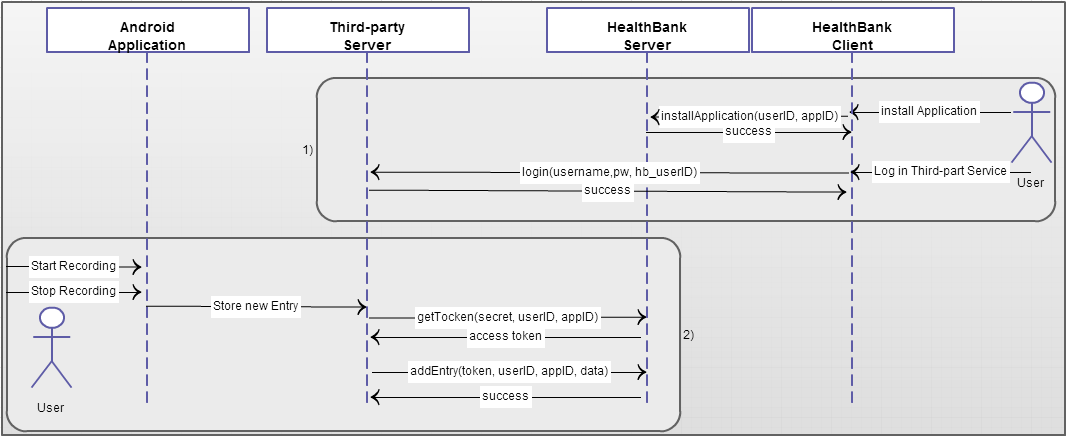
\includegraphics[width=355px,height=145px]{b2b.png}}%
\caption{Illustration of business to business communication to add new entry}
\label{fig:b2b}
\end{figure} 

As a first attempt to optimize for searching on the diverse field of data entries, we introduced index keywords. We ask the authors to provide these with the application information. Since applications have to store data in a key-value style, these index fields correspond to a set of keys which are most important to identify the record entry.

With this thesis we provide some initial applications. Most of them are rather basic and allow the user to upload simple health data via a form in the GUI. One application is particularly built for the users to add medical data. Another one is the equivalent for health care providers, which allows them to add medical data to a patient`s health record. There is an application for keeping record on the medications the users took. Two applications are part of a calories counter and allow calories intake with a food picker as well as calories burning with sports and daily calories consumption. Finally, an application is provided to keep track of endurance sports by providing the activity, duration, covered distance, heart rate etc.\newline
Following is a listing to give you an overview of how a record entry generated by for example the application to add medical data looks like on our database.

\begin{lstlisting}[language=json,firstnumber=1]
{
		"userID": "id",
		"app": "addRecord",
		"fileID": {
				"\$oid": "id"
		},
		"cause": "This is a test",
		"_id": {
				"\$oid": "id"
		},
		"timedate": "08/21/2013 14:23:47",
		"name": "File upload test",
		"fileName": "testFile.png",
		"descr": "This is a test to upload a file with a record",
		"doctor": "Dr. Test"
}
\end{lstlisting}


\subsection{Visualizations}

Visualizations are in many cases very similar to the applications defined above. They do also contain a name and a description, version number etc. Also they are defined in HTML / CSS / JavaScript files and are integrated to the GUI via an iframe. The main difference is the underlying concept. Visualizations are not allowed to add any data, but they can use the client API to access the entries of the space they are assigned to. This data can be used for drawing graphs etc. The most basic visualization, a simple list of the record entries, is present in every space page without the need of the user defining it initially. Next to this list, the user is allowed to add one visualization to each space, which will be integrated in an iframe on top of the list. When the page loads, the visualizations are able to get all the entries assigned to the particular space via a call to $parent.records$.

With the thesis we provide two initial visualizations. The first one is related to the two calories counter applications. It will search in the provided entries of the space, it is integrated to, for entries of one of the two applications. Then it uses these entries to build statistics about daily consumption and burning as well as overall data. The more it uses the Google Chart API~\cite{chartapi} to draw column charts. The second visualization is built for the endurance sports application and shows statistics about e.g. the total covered distance or duration. The more it illustrates the different attributes in graphs showing the progress over the latest entries.


\subsection{Messaging System}

The messaging system implemented for the prototype is rather basic and allows to send messages to only one other user at a time. A message contains a recipient, a header and the actual message. Users can access the messaging system either via the message icon in the action box on the very top of the screen or via the navigation link $inbox$. The message icon in the action box will change colour and begins to shake, when there are unread messages in the inbox. From the detail view of a message users can directly reply to it. Messages can be sent to any user in the system. There is no need for the users to have each other in its circles to send messages. 


\subsection{Queries}

Queries are executed only on the users and records of users that actively allowed researches to inspect their data. Therefore the query answers will not contain any data of users who did not set the research checkbox on the circles page. In the current prototype we implemented three types of search queries an institute user can use. In the following we describe these three types individually.

With a user query an institute can search for users by selecting certain constraints on e.g. the age, height, weight or the country the user lives in. In addition they can limit the search results by providing certain keywords which the record entries of the users shall contain. This query will help researches, if they search for users to participate in a certain study or similar. From the results list one can directly contact the users by the prototype`s messaging system. \newline
The second query type is used to search for certain records according to a set of keywords. This allows to search for symptoms of diseases, certain kind of injuries or similar. If there are multiple keywords separated by a space, the query performs a logical OR search on each keyword and returns record entries that contain any of the keywords.\newline
For the third type of search we used the new MongoDB text search. Since MongoDB version 2.4 they provide a text index which can be applied to all fields of a document that contain string values. Text search uses stop words, suffix stemming and is case-insensitive. With this framework we can ask queries with multiple terms (logical OR), by exact phrase searches (escape terms with quotes) and with negated terms (minus sign prefix). 

\subsection{Developer Guide}

Institutes can access the developer guide via the navigation in the apps part. The guide contains a documentation on all the services of the REST API running on the server as well as all the functions of the client-side API via JavaScript. The more we provided demos and all the information needed for creating new applications and visualizations. It has a separate design and is illustrated with code listenings and screenshots. 

\subsection{Security}

Even though security is a very important aspect for Healthbank, we did not emphasise too much on it. Nevertheless, there are a few points worth mentioning. 

We have already talked about our login and session management in chapter \ref{loginSession}. All passwords used for this process are stored encrypted in a MD5 hashed form on the database. We are aware of the fact that the MD5 hash function is severely compromised lately, but it still provides a sufficient amount of security for our purposes. The more, we never return the password hash to any client via a call to the REST API. 

We allow to upload many file types with record entries to our server. All of these files are stored directly in the MongoDB database. This is done to make sure that possible malicious files, which could harm the system, are not accessibly from outside and are never executed on the system itself. We used the GridFS specification for storing and retrieving the files in the database. GridFS was built to allow for storing files that exceed the BSON-document size limit of 16MB.

Authentication is disabled by default on MongoDB and we kept it that way for the process of implementing the system. However, MongoDB provides strong security, risk management strategies and access control~\cite{mongosecurity} which could be deployed if need be. 


%%% ------------- SECTION -------------
\section{Technologies}

In this section we describe the technologies we used to implement the different parts of the prototype. 


\subsection{Database}

As mentioned several times before, we used an instance of MongoDB~\cite{MongoDB} for our database. The MongoDB instance runs on the localhost on the same machine as the Tomcat server for the REST API. All the connections to the server run via the singleton class \verb+MongoDBConnector+ which implements our \verb+DBConnector+ interface. The interface includes queries, deletions, updates and insertions as well as methods to connect and set up the database. Because of the little data available for the prototype, we only used one server for now. Replication and sharding is documented very well on the MongoDB documentation website. Hence, it can be applied without too much effort as soon as the system is used by more users. For debugging we used the MongoDB shell tool, which allowed us to directly inspect and manipulate the database with the same queries as we used in the Java Servlets. As exemplified in the security section above, we omitted the authentication process on the locally running MongoDB instance for simplicity reasons. In the class \verb+MongoDBConnector+ of the backend the authentication is already prepared but still commented out. A description on how to apply a user name and password is present as well. All collection names, the host address and port of the database as well as the database name itself are loaded and parsed from a configuration file written in XML. 


\subsubsection{Indexes}
MongoDB defines indexes on a per collection level. Indexes can be set on single or multiple fields and are saved in a b-tree structure (see MongoDB documentation~\cite{MongoDBDoc}). Every collection has a default index on the $\_id$ field. To set our own indexes we are able to choose from a variety of options. MongoDB supports indexes on sub-documents and embedded fields as well as defining compound and multi-key indexes. We can set indexes to be unique, which guarantees, that the index field is unique, or to be sparse, where only records with this field defined will be indexed in the collection. Furthermore, there are hash as well as geospatial indexes and queries.

For our prototype we analysed the queries we ask most often and set a number of indexes to our collections to optimize for these queries. In the following list, we go through our collections and define the indexes we came up with:

\begin{itemize}
	\item Users collection: We do a lot of queries to the user name field of the user collection. Hence we set a secondary index on this field and set it to be unique, since we do not allow to set multiple user name fields. Hence in the user collection we have a total of two indexes, the standard index on the $\_id$ field and one on the user name field.
	\item Circles collection: Most of the queries to the circles collection use the $\_id$ field or the $userID$ field. Hence we set an additional index on the $userID$ field, so the database can decide, if the performance with the standard $\_id$ index is quicker than the one for the $userID$ field. Again we set the index to be unique, since obviously the userID for a circle has to be unique.
	\item Spaces collection: For the spaces the same as for circles applies. Hence we set an additional index on the $userID$ field.
	\item Messages collection: On the messages collection we set a compound index on the $senderID$ and $recipientID$ fields since this allows to optimize queries for the communication between two users. 
	\item News collection: For the news collection we did not set any additional indexes. Most of the queries use the $\_id$ field, the more the amount of news entries to expect is rather low compared to other collections.
	\item Applications collection: We set a compound index on the fields $userID$ and $appID$. This shall speed up queries to installed applications and during the (un)installing process. For requests to applications we usually use the $\_id$ field and hence, we need no additional index.
	\item Record collection: Apart from the standard $\_id$ index, we also set one to the $userID$ field since many queries use this field. Again we set it to be unique. In addition, we set a text index on all fields of the collection for the text search query defined above.
\end{itemize}


\subsection{Server}

On the server we used Java Servlets~\cite{JavaServlets} to implement the REST API and the MongoDB Java Driver~\cite{mongoJavaDriver} to get a connection to the database. There are eighteen servlets in total in the prototype so far, each defining individual functionalities accessed via HTTP GET or POST requests. The more, there is a \verb+DBConnector+ interface with an implementation for MongoDB, that handles the connection and queries to the database, as well as a \verb+CoreManager+ class, that deals with core functionalities used in multiple servlets. File manipulation and hashing for security aspects was done with the help of libraries from the Apache Commons project~\cite{apachecommons}. For parsing JSON data we used the JSON.simple framework~\cite{jsonsimple}. During the implementation we worked with Eclipse and deployed the servlets on a Tomcat server version 7.0 on Windows 7. For testing purposes and to make it publicly available we deployed the WAR file on a Tomcat server running on an ETH Debian server.

\subsection{GUI for Client}

The client is completely decoupled from the server side and runs on any kind of HTTP server such as an Apache or Tomcat server. It consists of a number of HTML, CSS and JavaScript files. Common components such as the navigation or the action box on the top right of the screen are loaded dynamically from a common source. When we change these components this brings the advantage of less copy and paste for the individual files. For Document Object Model (DOM) manipulation and other useful features we used the JavaScript library jQuery~\cite{jQuery} and the jQuery UI plugin. 
\newline
For every page we use a single HTML file. Since the GUI has become rather big over time, we favour this solution in contrast to a single page architecture, such as solution built with the Google Web Toolkit~\cite{gwt} or similar. All these pages share the $healthbank.js$ JavaScript file and $healthbank.css$ cascade style sheet. We tried to put all the JavaScript code into a single file to reduce the overall amount of files to be loaded by each request. When the DOM of any page is loaded we first call the $initialize()$ JavaScript function. This function includes loading the correct navigation and action box, querying user profile data, checking for new messages and the like. Then we load the actual content for the page. Whenever appropriate, we added some animations and transitions using the new CSS capabilities. This shall give the page a more modern view and interactions the users are familiar to. Dialogs and pop-up menus are often loaded dynamically, so we can reuse as many of them as possible (e.g. menu for adding circles and spaces). \newline
For the developer guide, which serves as the documentation for the prototype, we used a different design then on all the other pages. Navigation is still on the left but there is no action box and user related content. This design is rather simplistic and static and is loosely based on automatically generated Java Doc HTML pages.

\textbf{Communication} \newline
The communication with the server was done using AJAX (Asynchronous JavaScript and XML) requests who call the server REST API. Apart from the login, which is dealt with separately, all of these AJAX request are defined in the $healthbank.js$ JavaScript file. The REST API so far only supports GET and POST requests. With the help of jQuery the requests are rather straight forward and contain the data to send, the type (POST, GET), the URL and the data type to deal with. The response is mostly provided in a JSON structure. Most of the responses provide, next to the data, information about, if the session is still active and if the call was successful or not. In case of a success the \emph{values} field contains the desired data (e.g. an array of record entries), in case of an error the \emph{error} field contains the error message. When the session key is expired or the credentials are wrong, the functions will automatically redirect the user to the login page and no data is returned. In the following listening we illustrate a successful followed by a failed request to the user query.

\begin{lstlisting}[language=json,firstnumber=1]
{
    "result": "success",
    "loggedOut": "false",
    "message": "Here are the results.",
    "values": {
        "users": [
            {
                "userId": {
                    "$oid": "id"
                },
                "userIcon": {
                    "$oid": "id"
                },
                "lastname": "Tremp",
                "firstname": "Patrick"
            }
        ]
    }
}
{
    "result": "failed",
    "loggedOut": "true",
    "error": "Either your session timed out or you forgot to send me the session and credentials."
}
\end{lstlisting}



%%% Local Variables:
%%% mode: latex
%%% TeX-master: "thesis"
%%% End: